\scanpage{113}

\uline{Bertini's theorem and variants}.

In what follows $k$ denotes a field, $P^r=P^r_k$.

\margin{\figure{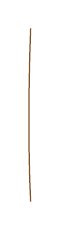
\begin{tikzpicture}\draw[brown!65!black,line width=.45pt] (0,0) .. controls (-.03,-.8) and (-.03,-1.6) .. (0,-2.2);\end{tikzpicture}}}
\uline{Bertini's theorem} 1: Let $f:X\handwritten{\rightarrow}P^r_k$ be a morphism, where $X$ is a geometrically irreducible algebraic scheme, and let $n=\dim\overset{\handwritten{\rule{1.9em}{.4pt}}}{f(X)}$. Let $L_t$ be the\deleted{\unsure{s|a}} \uline{generic} linear subspace of codimension $s$ of $P^r$, where $s$ is a fixed integer $\handwritten{\leqslant}n-1$. Then $\inserted{Y_t=}f_t^{-1}(L_t)\handwritten{\subset}X_t=X\otimes_k k(t)$ is geometrically irreducible.

\margin{\handwritten{\unsure{true} in\\\unsure{E|S}GA \unsure{V|IV}}\figure{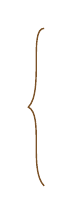
\begin{tikzpicture}\draw[brown!65!black,line width=.5pt] (.2,0) .. controls (0,0) and (.2,-.8) .. (0,-1) .. controls (.2,-1.1) and (0,-1.8) .. (.2,-2);\end{tikzpicture}}}
\margin{\figure{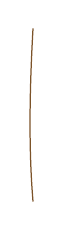
\begin{tikzpicture}\draw[brown!65!black,line width=.45pt] (0,0) .. controls (-.04,-.7) and (-.06,-1.5) .. (0,-2.2);\end{tikzpicture}}}
\inserted{Local statement 2: Let $f:X\handwritten{\rightarrow}P^r$ be a morphism, with $X$ an algebraic scheme.} \deleted{\uline{Complement}\unsure{:} Suppose} Let $Z\handwritten{\rightarrow}X$ \deleted{\illegible{2}} be the set of points of $X$ at which \inserted{\handwritten{either}} $f$ is \deleted{\handwritten{either}} ramified \deleted{or at which} \inserted{\handwritten{or}} $X$ is not geometrically unibranch (resp.\ \inserted{\handwritten{not}} normal, resp.\ \inserted{\handwritten{not}} smooth \ldots), \deleted{then} and suppose that $\overset{\handwritten{\rule{1.9em}{.4pt}}}{f(Z)}$ has dimension $\handwritten{<}s$. Then $\inserted{Y_t=}f_t^{-1}(L_t)$ is geometrically unibranch (resp.\ normal, resp.\ smooth \ldots), where $L_t$ is as above.

From these two statements one deduces\handwritten{/}formally;

\margin{\figure{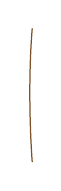
\begin{tikzpicture}\draw[brown!65!black,line width=.45pt] (0,0) .. controls (-.05,-.6) and (-.03,-1.3) .. (0,-1.7);\end{tikzpicture}}}
\deleted{Theorem}\uline{Corollary} 3: Let $f:X\handwritten{\longrightarrow}P^r$ satisfy the conditions of 1\handwritten{,} and 2 non respé.\ \inserted{Suppose $k$ algebraically\ closed.} Then \unsure{the|the}\deleted{inclusion} canonical morphism
\[
\handwritten{\pi}_1(Y_{\bar{t}})\handwritten{\rightarrow}\handwritten{\pi}_1(X)
\]
is surjective.

\uline{Re\unsure{ma}\unsure{r|q}k} \unsure{3|4}. Using the base change theorems for $\handwritten{\pi}_1$, one concludes \deleted{that} (putting $X_{\bar{t}}=X\otimes_k k(\bar{t})$) that the homomorphism $\deleted{\unsure{\pi}_1(}$
% The written display label is at the left margin.
\[
\handwritten{\pi}_1(Y_{\bar{t}})\handwritten{\rightarrow}\handwritten{\pi}_1(X_{\bar{t}})\tag*{\makebox[0pt][r]{\makebox[\linewidth][l]{(*)}}}
\]
is surjective if $X_{\deleted{\unsure{t|\bar{t}}}}$ is proper, and that the homomorphism
% Both X- and Y-like contours occur in the source cell; no correction order is established.
% The written display label is at the left margin.
\[
\handwritten{\pi}_1^{!}(\unsure{X|Y}_{\bar{t}})\handwritten{\rightarrow}\handwritten{\pi}_1^{!}(X_{\bar{t}})\tag*{\makebox[0pt][r]{\makebox[\linewidth][l]{\handwritten{(**)}}}}
\]
is surjective, where the ! denotes the largest profinite quotient prime to the characteristic\ e\unsure{d|x}ponent of $k$. One does not assert, however, that (*) is always surjective (without a properness hypothesis on $X$).

One deduces, from 1, by an easy application of the connectedness theorem:

% The second marginal numeral retains the V/IV ambiguity first marked in the upper note.
\margin{\handwritten{seen.\ in\\EGA V}\figure{\begin{tikzpicture}\draw[brown!65!black,line width=.45pt] (0,0)--(.03,-.5);\end{tikzpicture}}}
\uline{Corollary} 4 (of 1): Under the conditions of 1) for $f:X\handwritten{\longrightarrow}P^r$, if $X$
% archive sheet number: 112
